%!TEX root = ../report.tex

\begin{document}
    \chapter{Related Work}


    \section{End-to-End Autonomous Driving}
    The landscape of end-to-end autonomous driving based approaches can be divided based on the different learning methods used like imitation learning, reinforcement learning, transfer from simulation to real world via generative adversarial learning.
This section will briefly discuss some of the contribution in the field of end-to-end autonomous driving. A vast amount of work has been carried out via imitation learning in simulated and real wold environments. 
\par Testing of imitation learning techniques are categorized under closed loop and open-loop evaluation. In open-loop evaluation an autonomous driving model is compared to the recorded expert driving behavior, where the training data is generally split into test and train and the evaluation is carried out on test data. Popular open-loop evaluation metrics are Mean squared error, Mean absolute Error. Whereas in closed loop evaluation the evaluation is carried out in a real driving scenario in which a driving model is made to control the car. Evaluation metrics used for closed loop testing found in the literature are like percentage of autonomy, number of disengagements, number of infractions like collisions, average distance between disengagement and infractions.

 \begin{figure}[h]
    \centering
    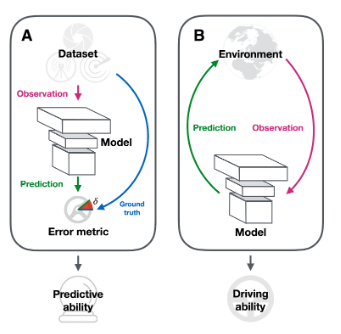
\includegraphics[width=6cm, height=5cm]{images/open_closed.png}
    \caption{Open and closed loop evaluation in end-to-end autonomous driving \cite{DBLP:journals/corr/abs-2003-06404}}
    \end{figure}

\cite{DBLP:journals/corr/BojarskiTDFFGJM16} PilotNet by NVIDIA is one of seminal papers in end-to-end learning for self driving cars. Where a convolutional neural network is trained with images from a single front facing cameras to predict steering commands.  This work made the researchers to believe in the power of end-to-end imitation learning. \cite{DBLP:journals/corr/abs-1711-03938} released a benchmark called CARLA for testing and developing autonomous driving solutions. \cite{DBLP:journals/corr/abs-1710-02410} proposed a conditional imitation learning based approach where steering and acceleration commands are obtained from the neural network model trained on images from a front facing camera mounted on a toy-truck, navigation commands are treated as intermediate inputs to the network after feature extraction and intensive exploration of closed and open-loop metrics is carried out.

\cite{Sobh2018EndToEndMS} proposed a multi-modal fusion of camera and a lidar BEV segmentation along with navigational commands to predict steering and throttle. This work can be seen as multi-modal extension of conditional imitation learning. Conditional affordance learning \cite{DBLP:journals/corr/abs-1806-06498} introduced the importance of affordances in the environment to take driving decisions. They predicted different kind of affordances like distance to center line of the road, traffic light sign and speed limit affordance with respect to a safe area along with navigational commands to make decisions. Along with that they also developed a control algorithm to take away the jerky car motions for real time applications. 

\cite{DBLP:journals/corr/abs-1804-09364} bridges the gap between end-to-end and modular approaches via abstraction by predicting semantic maps from images and using those semantic maps for obtaining driving commands. \cite{DBLP:journals/corr/abs-1807-03776} proposed principled controllable imitative reinforcement learning which is a combination of imitation and reinforcement learning, where the Deep Deterministic Policy Gradient is used to boost the generalisation of the driving policy. \cite{DBLP:journals/corr/abs-1803-10158} used surround view cameras, vehicle canbus data along with images from open street map to predict driving commands and provided their own large scale dataset called drive 360. They have introduced the usage of LSTM's to capture the temporal information from the scene. Chauffer Net \cite{DBLP:journals/corr/abs-1812-03079} used top down representation of the scene obtained from a perception stack to predict trajectories of the ego vehicle and those trajectories are processed by planner module to give driving commands. 

\cite{DBLP:journals/corr/abs-1905-12887} conducted controlled experiments to show that explicit intermediate visual representation play a major role in predicting actions. \cite{DBLP:journals/corr/abs-1906-03199} proposed a multi-modal conditional imitation learning approach where they used monocular and depth images along with speed measurements to predict actions. \cite{DBLP:journals/corr/abs-1903-10995} proposed a way to learn accurate and comfortable human like driving  using adversary learning. \cite{DBLP:journals/corr/abs-1912-00177} proposed an approach based on conditional imitation learning using images from multiple views, where each image is passed through a CNN based feature extraction module and fused. Those fused features and navigational commands are used to predict driving commands. They have used the intermediate features to predict semantic segmentation, monocular depth and optical flow. 


\cite{DBLP:journals/corr/abs-1904-08980} explored the limitations of conditional imitation leaning regarding data set biases, training instability and the ability of the learned driving policy to not perform well in unseen environments. \cite{DBLP:journals/corr/abs-2101-06679} proposed a neural motion planner to drive autonomously in urban scenarios, which includes traffic-light handling, yielding and interaction with multiple road users. They have used Lidar and Hd maps to produce intermediate representations in the form of 3D object detection and trajectory prediction. \cite{Casas_2021_CVPR} provides a novel idea of map-less driving where they are generating an online top down representation of the scene and not relying on the HD maps. Along with that interpret-able intermediate results are predicted for the dynamic objects in the scene. A motion planner module extracts the features from the previous stage to predict actions. In motion planning module possible trajectories are obtained via dynamic occupancy field based trajectory sampler and all the aggregated features are passed into a cost function to predict a desired vehicle trajectory. 

Recent trends in self driving is moving towards an idea where they have assumed that their perception outputs are quite accurate. And they are relying on the those perception outputs like 3D object detection, semantic segmentation, monocular depth prediction, monocular BEV segmentation to generate top down representation of the scene not relying on lidar and HD maps. After that a motion planning module is used to make the decisions. The whole pipeline is generally trained in an end-to-end fashion. Lift, Splat Shoot \cite{DBLP:journals/corr/abs-2008-05711} by NVIDIA is a very good example of the same. Recently a company called CommaAI released a device for advance driver assistance system and along with that their software stack which is open sourced. The neural network architecture used for driver assistance outputs 10 various outputs like lane-lines, road edges, paths, lead car prediction, pose and various other meta information responsible for driving assistance using only the monocular image captured by a dash cam from the device. 

Even after the vast research in the field of end-to-end autonomous driving we are still far away from achieving full self driving and the approaches still suffer from the problem of causal confusion, generalisation in different scenarios and other challenges as described in section 1.1. Very minimal amount of work has been done which is focused towards task loss balancing, finding an appropriate unified feature extractor. Auxiliary tasks like predicting lane lines, paths, road edges, dynamic objects, monocular depth, BEV semantic segmentation seems to be beneficial for predicting actions.

%--------------------------------------------------%
    \section{Multi-task Learning Vs Auxiliary Learning}
    
    In this section we will briefly understand the meaning of multi-task learning and what role it can generally play in autonomous driving, by mentioning some approaches related to the same. 
    
    In machine learning in general we typically try to learn for a task by minimizing on an objective function, thus quantifying an approach with respect to some metrics by training a single model. We can fine-tune our trained model to generalize well and modern deep neural networks are really effective in learning one task and have achieved great results in the field of computer vision \cite{DBLP:journals/corr/KaiserGSVPJU17} \cite{DBLP:journals/corr/abs-1904-08492}, natural language processing \cite{DBLP:journals/corr/KaiserGSVPJU17} and speech recognition \cite{DBLP:journals/corr/ToshniwalTLL17} more. Generally we focus on optimizing for one task and ignore the other information which can be beneficial for the model in terms of training signals to optimize the metric even better and those training signals can be obtained by training for related tasks. Thus by sharing the feature representation between various related tasks we can optimize the metric even better, this way of learning is termed as multi-task learning. 
    
    Biologically, human way of learning completely overlaps with multi-task learning. As we use the knowledge acquired during learning previous tasks to learn new task. Like a baby first learn to recognize faces and then further using this learned representation to decipher certain objects. Researchers have also accounted multi-task learning for introducing inductive bias in the machine learning which can prevent over-fitting and leads to better generalization. Generally this inductive bias is introduced by the learning of auxiliary task along with the main task. Any problem where you are optimizing more than one loss function can be categorized as multi-task learning. 
    
    By definition both auxiliary learning and multitask learning is same, in both the cases you are learning for multiple tasks by sharing the feature representation thus utilizing the training signals from related tasks, the only difference is that in auxiliary learning the other tasks are non operational with respect to the main task. The auxiliary task is general trained on more annotated data to act as a regularizer for the main task. 
    
    In Autonomous driving, multi-task learning or auxiliary learning plays a very important role. For example if we talk about a scenario where a car is driving on a busy street. So, for an autonomous car to make decision in this scenario we need to learn for tasks like road sign detection, object in closest path, curbs, moving objects, traffic lights and more. Some of these tasks share some correlation and to exploit that we need to learn them together. Multitask learning or auxiliary learning faces a lot of challenges and difficulties like we need to select a unified feature extractor for all the tasks \cite{DBLP:journals/corr/abs-2108-11353}, choosing the appropriate architecture for a multitask system followed up by which parts of the network should be share by the which tasks \cite {Liu_2020_ACCV} \cite{ruder2018latent} \cite{DBLP:journals/corr/abs-1904-02920}, which tasks needs to chosen for multitask learning \cite{DBLP:journals/corr/abs-2110-07301} \cite{DBLP:journals/corr/abs-1904-04153}, how to jointly train multitasks such training signals from other tasks helps main task \cite{DBLP:journals/corr/abs-1903-12117} \cite{DBLP:journals/corr/abs-2007-06889} \cite{DBLP:journals/corr/abs-2001-06782} \cite{Guo_2018_ECCV}, balancing the losses for optimizing various tasks such that it can enhance the efficiency of the main task \cite{DBLP:journals/corr/abs-1904-08492} \cite{pmlr-v80-chen18a} \cite{du2020adapting}. So all of these challenges are in itself a separate area of research in machine learning. 
    
    In \cite{DBLP:journals/corr/abs-1805-06334} semantic segmentation is carried out where as prediction of time and weather is used as auxiliary tasks. \cite{teichmann2018multinet}, \cite{7785137} conducted joint learning of semantic segmentation and depth estimation as both task share some meaningful information, have shown that learning depth estimation has auxiliary task has leads to increase in performance. \cite{yang2018endtoend} jointly learned for prediction of driving commands in terms of steering angle and speed in end-to-end fashion. \cite{Wang2019EndtoEndSU} explored to predict the driving commands with object detection and semantic segmentation as auxiliary tasks. \cite{9090850} proposed a lightweight based network using Lidar as main sensor to predict the occlusion free road segmentation, road ground height estimation and road topology recognition with keeping later two as auxiliary tasks. \cite{teichmann2018multinet} jointly learned classification, detection and semantic segmentation of scene objects for semantic reasoning using a unified feature extractor and task specific decoders. In \cite{9523129} driving commands are predicted along with monocular depth estimation, semantic segmentation and traffic light state as auxiliary tasks. 
    
    Along with inducing inductive bias and inducing task related information which is missing in the main task multi-task learning also helps in creating interpret-able solutions. Any failure in the main task can be validated via the output from sub-tasks and vice versa. So multitask learning is a main component of end-to-end autonomous driving or autonomous driving.  

%-----------------------------------------------------%
    \section{Lane Detection in Autonomous Driving}
    Lane line detection is one of the most fundamental and safety critical task in autonomous driving. The importance of lane line detection varies from ADAS (advanced driver-assistance systems) to powerful autonomy tasks like fusion with HD maps and trajectory planning.
        %==============================================%
        \subsection{Monocular 2D Lane Detection}
        Traditionally lane detection was carried out using hand crafted features. Those approaches have many drawbacks like lack of robustness, only applicable in easy driving scenarios. Recently deep learning techniques has been employed to remove the reliance on the hand crafted features and to extract those features in an end-to-end fashion. 2D lane detection requires to capture rich context from the scene, as in most of the scenarios we need to face challenging situations where there are no lane markings, lanes markings are occluded by the objects or extreme lightning and weather conditions. Thus thus we need to counter the biggest problem of missing visual cues in the scene, maintaining the real time applicability of the solution.
        
        The task of lane detection via deep learning is generally considered a dense prediction task of semantic segmentation, where each pixel in an image define a label whether it is a lane or not. Semantic segmentation in general is considered as dense prediction task, so to facilitate that we need to increase the effective receptive field. To Support that \cite{DBLP:journals/corr/abs-1712-06080} proposed a feature enhancement module which can be used flexibly after the initial feature encoding in any model and shown to be faster than Deep Lab V3 \cite{DBLP:journals/corr/ChenPSA17} and lesser number of parameters. Following the previous approach RESA \cite{DBLP:journals/corr/abs-2008-13719} proposed a better feature enhancement module and at the stake of less computational cost, resulting in 10 times faster than the predecessor. 
        
        As the task of semantic segmentation involves around predicting the accurate class of the pixel, approaches like \cite{https://doi.org/10.48550/arxiv.2010.12035}, \cite{inbook} have shown that predicting a semantic mask does not solve the problem of defining shapes of the lane lines, therefore anchor based and row-wise detection based 2d lane detection methods were proposed.
        
         \begin{figure}[h]
    \centering
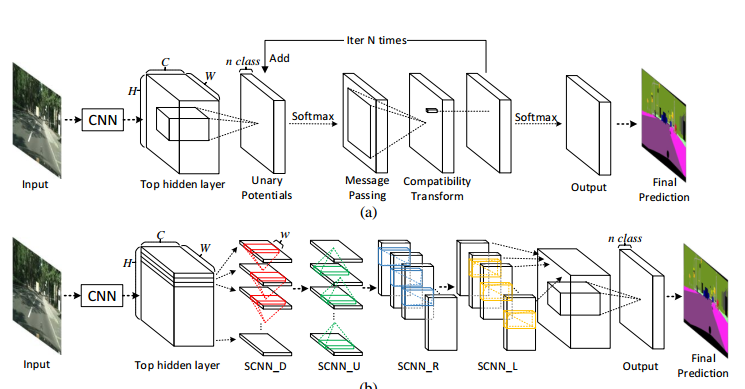
\includegraphics[width=12cm, height=4cm]{images/scnn_module.png}
    \caption{SCNN: feature enhancement module proposed by  \cite{DBLP:journals/corr/abs-1712-06080}}
    \end{figure}
    
     \begin{figure}[h]
    \centering
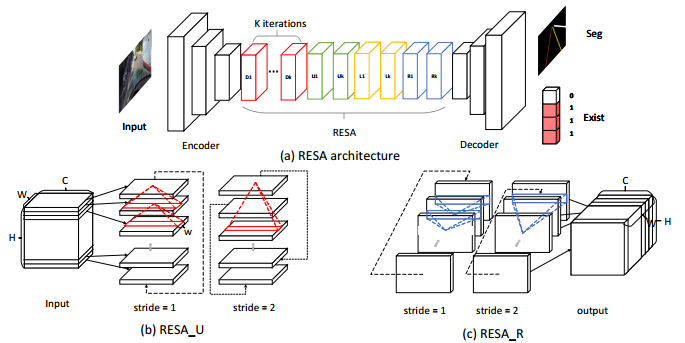
\includegraphics[width=12cm, height=4cm]{images/resa_module.png}
    \caption{RESA: feature enhancement module proposed by \cite{DBLP:journals/corr/abs-2008-13719}}
    \end{figure}

 Approaches like \cite{DBLP:journals/corr/abs-2005-08630}, \cite{DBLP:journals/corr/abs-2004-11757}Monocular 3D Lane Detect employed row-wise classification methods to detect lane lines. In row wise detection methods, an image is divided into a grids and a neural network model predicts the most probable cells which can contain part of the lane lines. Generally some post processing methods are used to obtain lane lines like clustering. Although row wise classification have proven to better in terms of efficiency and accuracy but these approaches still suffer from instance level discrimination of predicted lane pixels.
 
 Anchor based approaches like  \cite{https://doi.org/10.48550/arxiv.2010.12035} try to counter the missing vision cue problem by using predefined anchors and regressing the lane coordinates on the basis of predefined anchors but fixing the anchors shapes are shown to be a restriction in describing the lane shapes.

Several methods have been proposed to capture the rich context of the scene via multitask learning like \cite{inbook} and it has been proven that these methods lead to gain in the performance but it comes with it cons like multi task learning based approaches require extra annotations and large inference times. Some knowledge and attention distillation based approaches have also been proposed to tackle the aforementioned challenges like \cite{DBLP:journals/corr/abs-1908-00821}. Some approaches like PolyLaneNet\cite{DBLP:journals/corr/abs-2004-10924} have tried  to represent a lane-line by a polynomial and tried to directly regress the parametric representation of the lane curve equation. So far parametric based methods are not able to exceed the other methods in terms accuracy.

Row wise detection based or anchor based methods for 2d lane detection are better in terms of accuracy and inference time, but we speculate that segmentation based approaches are mainly using ResNet\cite{DBLP:journals/corr/HeZRS15} based architectures for initial feature extraction. As \cite{DBLP:journals/corr/abs-2105-05003} has shown that there can be a possibility of extracting even richer context from the scene using self-attention based feature encoder like transformers \cite{https://doi.org/10.48550/arxiv.1706.03762}.   SAN\cite{DBLP:journals/corr/abs-2004-13621} and SENet\cite{DBLP:journals/corr/abs-1709-01507} are also one of the attention based feature extractor modules which can be explored for feature extraction which have proven to be better than traditional ResNet\cite{DBLP:journals/corr/HeZRS15} in terms of number of parameters and accuracy. 

So in general 2d lane detection algorithms take an RGB image from a camera mounted on autonomous vehicle, and provides set of lines on that image. Those lines are projection of 3D lane lines on the image. As both input and output are represented in the image space that is why such approaches are called 2D. These approaches assumes that the road plane is flat and in scenarios where the roads are with different alleviation, there exists a need to obtain 3D points of the lanes to perform accurate motion planning. This work mainly relies on detecting 2d lanes via semantic segmentation which facilitates our 3D lane detection approach which will be discussed in the further sections. 
        
        %==============================================%
        \subsection{Monocular 3D Lane Detection}
        Monocular 3D lane detection system provides real world 3D coordinates of the lane lines with respect to a camera coordinate system. This field is quite new and some efforts have been recently done in exploring this task. 
 
The most basic way to lift the 2d lane lines to 3D is using Inverse perspective mapping. IPM is a homographic transformation which warps a perspective image to birds eye view (BEV). But the main problem with IPM is that it assumes flat ground followed by a static and well calibrated camera, where as in real world scenarios the roads are rarely flat. One possible way to predict 3D lanes might be via predicting monocular depth maps of the scene and associate each point of the lane line with depth. Although such solution can be resource hungry we need a light weight and real-time working solution. Apart from that monocular 3D lane detection has a relationship with other tasks like monocular 3D object detection, Monocular BEV segmentation in terms to recover 3D information of the scene using a monocular image.
\cite{DBLP:journals/corr/abs-1802-05591} is a 2D lane detection approach and many of its idea formed a corner stone for the existing 3D lane detection based approaches. The authors have proposed a lightweight network called H-Net to predict the homo-graphic transformation directly from the image. They took two basic assumptions in their approach that every lane line can be represented by a 3rd order polynomial and lane lines are on a flat road. 

 \begin{figure}[h]
    \centering
    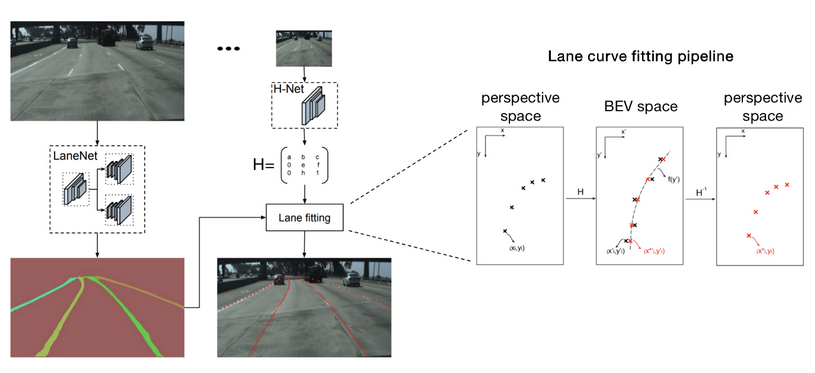
\includegraphics[width=\textwidth]{images/lanenet.png}
    \caption{Pipeline of \cite{DBLP:journals/corr/abs-1802-05591}}
    \end{figure}


The most seminal paper in the field of 3D lane detection is \cite{DBLP:journals/corr/abs-1811-10203} like \cite{DBLP:journals/corr/abs-1802-05591} they have not taken any flat ground assumption, the architecture in the approach is basically divided into two pathways one for predicting the transformation from image plane to 3D road plane. This pathway predicts camera height and pitch from the road which basically determines the transformation. The other pathway is responsible for converting monocular image from image space to Bird-Eye-View (BEV) space, where they have employed an anchor based lane prediction head. The main limitation of this approach is that it can handle only scenarios with parallel lane-lines and fail at the scenarios when lane-lines are perpendicular to the ego vehicle. 

\begin{figure}[h]
    \centering
    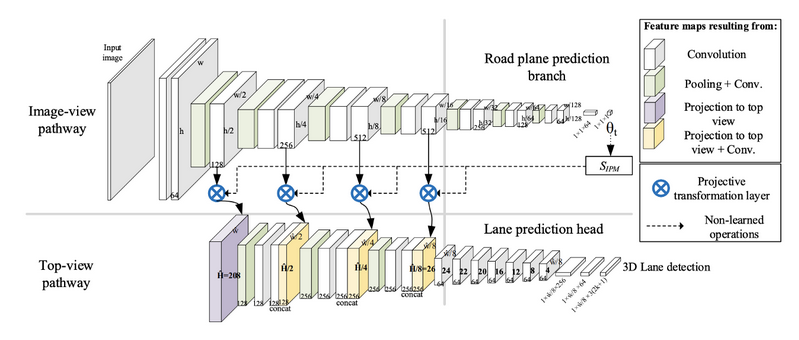
\includegraphics[width=\textwidth]{images/3dlanenet.png}
    \caption{\cite{DBLP:journals/corr/abs-1811-10203} 3D LanetNet network architecture}
    \end{figure}

\cite{DBLP:journals/corr/abs-2011-01535} handles the limitations of \cite{DBLP:journals/corr/abs-1811-10203} and like its predecessor it has also similar dual pathways but the only difference is the representation of the lane lines. It breaks the BEV image into grids called image tiles.
Every lane segment passing through each tile is approximated semi-locally and constructed into a full lane curve, moreover this is the first work where they have also introduced estimation of uncertainty for 3d lane detection. This paper also claims that it is able to handle the scenarios with different topologies as their method encode 3d lane information with anchor-less 3D lane representation. 

 \begin{figure}[h]
    \centering
    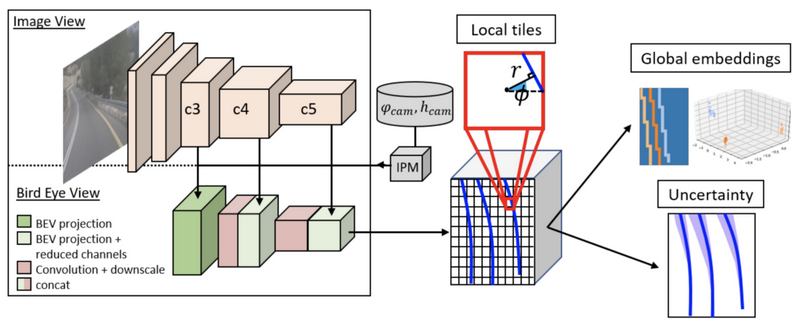
\includegraphics[width=12cm, height=4cm]{images/3DLaneNET++.png}
    \caption{Network architecture of Semi-local 3D LaneNet \cite{DBLP:journals/corr/abs-2011-01535}}
    \end{figure}

\cite{guo2020gen} also proposes a two stage method to predict 3D lanes. In the first stage they perform 2D lane detection and in the next stage they lift the 2d lane detection results to 3D using a different network which they have called as 3D-GeoNet. The main important thing about this approach is the first stage can easily be replaced by better 2D lane detection algorithms and. They have treated lane detection and prediction of 3D geometry as different tasks thus making their approach even more flexible and moreover the second stage is trained with synthetic 3D lane detection dataset that they have released along with the original implementation of the approach. 

 \begin{figure}[h]
    \centering
    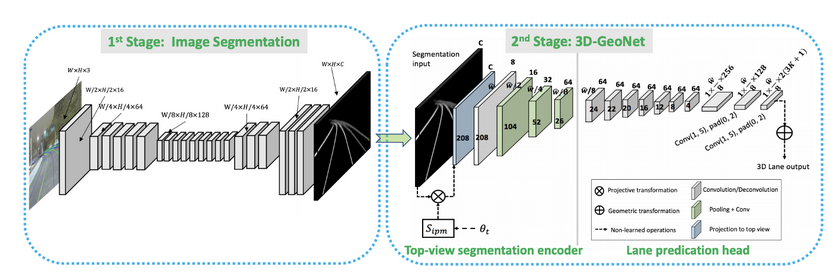
\includegraphics[width=\textwidth]{images/GenLaneNET.png}
    \caption{Network architecture of Gen-LaneNet \cite{guo2020gen}}
    \end{figure}

The authors have also pointed out more limitations of the \cite{DBLP:journals/corr/abs-1811-10203} that in case of a scenario when a ego vehicle is moving uphill the top view projection does not align with IPM transformed projection, thus the IPM transformed features are warped which they call it is as virtual top view. All the 3D lane line ground-truths are corrected to virtual top view before feeding it into the model. Despite of many improvements this approach has used anchor based representation of the lane lines thus they suffer from the same limitations as \cite{DBLP:journals/corr/abs-1811-10203}. 

All the previous mentioned approaches for 3D lane detection are relying on accurate camera poses in terms of camera height and camera pitch. \cite{DBLP:journals/corr/abs-2112-15351} are performing the task of camera pose prediction and determining 3d lane lines. They have divided their network to two stages. The image input to the network is processed by convolution neural network followed by a transformer-encoder inspired by LSTR \cite{LSTR}. Instead of representing the lanes in the form of anchors the lanes are represented in the form of multi order polynomial and their coefficients are regressed in the training. They have explored the fact of predicting camera pose, as the previous work fails on high speed and high undulations. Though this approach performs better in terms of metrics but they are still unable to take into account the problem of detecting 3d lane lines for complex topologies. 

 \begin{figure}[h]
    \centering
    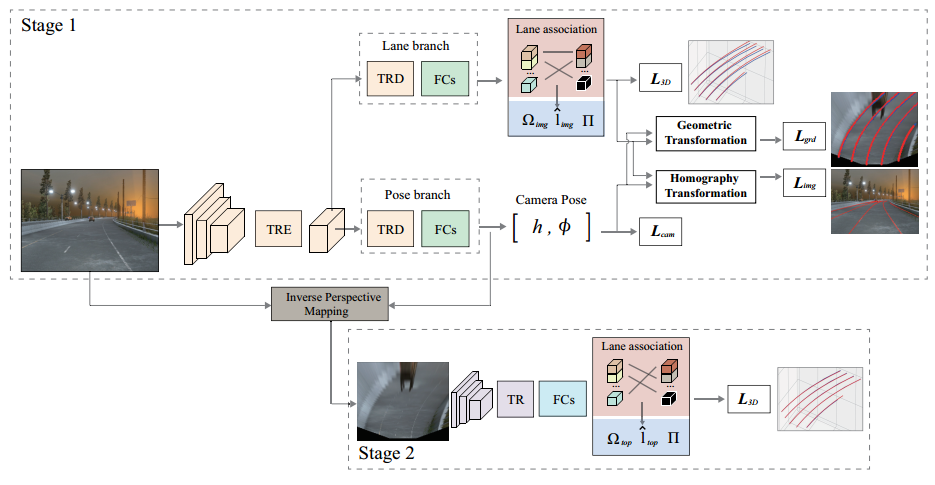
\includegraphics[width=\textwidth]{images/3dLane_camera_pose_pipeline.png}
    \caption{Pipeline of \cite{DBLP:journals/corr/abs-2112-15351}}
    \end{figure}

Following the previous work \cite{9506296} proposed a dual attention pipeline for 3d lane detection. Their dual attention is itself a flexible contribution which can be replaced in any other approach. The main essence of dual attention module is to extract more meaningful global information. In this approach the output feature map from the segmented BEV is further processed via fully connected layers to find the correction between the lane anchors in horizontal and longitudinal fashion this extraction lane-to-lane and pixel wise attention. The global attention map or features are used for predicting 3d lanes. Thought their dual attention module is interesting but it is utilizing anchors to represent 3D lane lines thus this approach will suffer from the same limitations as we have discussed above. 

 \begin{figure}[h]
    \centering
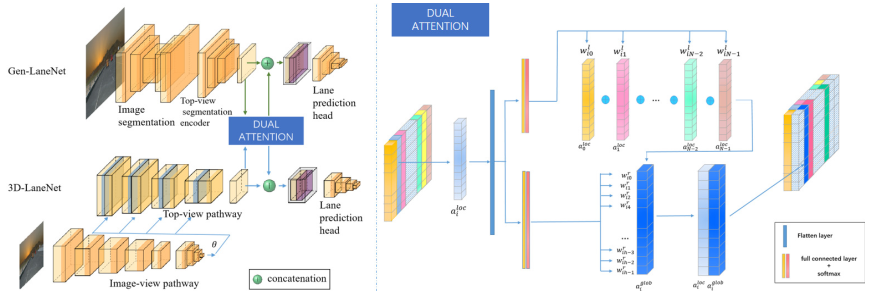
\includegraphics[width=12cm, height=4cm]{images/dual_attention_pipeline.png}
    \caption{Dual attention mechanism  proposed by  \cite{9506296}}
    \end{figure}

Following the footsteps of \cite{DBLP:journals/corr/abs-2011-01535}, \cite{yan2022once} proposed a lane detector where lanes are not represented as anchors. Instead of using BEV for encoding 3d lane information the scene their method relies on the 2D camera image and its intrinsics to detect the 3D lane line points. Utilizing the power of anchor-less based 3d lane detectors that they are able to detect different lane topology, they have used a dual branched pipeline where one branch is used for detecting binary lanes from the encoded features from a input image. For the backbone they have used the SegFormer \cite{DBLP:journals/corr/abs-2105-15203}. The second paths regresses directly the 2d coordinates of the lane points along with the depth associated with them. The predicted coordinates are in camera image plane which can be taken to real world via using camera geometry. For generating the ground-truth they have proposed an automatic annotation pipeline using Lidar and camera as major sensors.

\begin{figure}[h]
    \centering
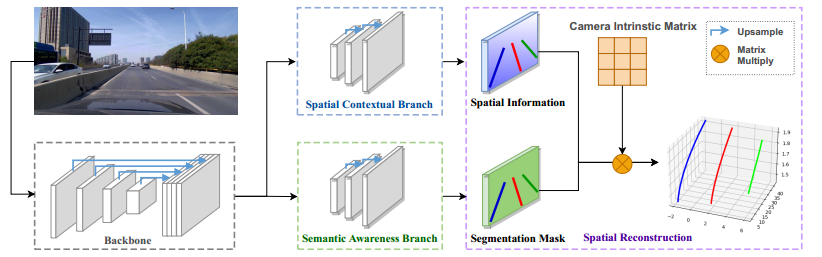
\includegraphics[width=12cm, height=4cm]{images/once_pipeline.png}
    \caption{Extrinsic free anchor-less pipeline proposed by \cite{yan2022once}}
    \end{figure}

In this work we propose to take the best of the both the worlds and counter the limitations of the previous approaches by using virtual top view and decoupled pipeline proposed by \cite{guo2020gen} and using the tile representation opted by \cite{DBLP:journals/corr/abs-2011-01535}. We will also explore the flexibility of the dual pathway in terms of using more complex lane segmentation solution.

\subsection{Lane Detection Datasets}
This section introduces the reader to popular 2D and 3D public lane detection datasets used for this work and by the research conducted in the respective field. 

\subsubsection{2D Lane Detection Datasets}
As a lot of work has been conducted in the field of 2d lane detection therefore a lot of 2d lane detection data-sets exits. But in this work we will discuss only the prominent ones which are generally used by the 3D lane detection approaches for training the intermediate part of their pipline. \cite{Tusimple} TuSimple is one of the most basic datasets used by the 2d lane detection approaches to validate their pipeline. The dataset consists of driving scenarios on highway with stable lightning conditions. Where as CULane \cite{pan2018SCNN} is quite challenging dataset with varying driving conditions. The dataset consists of 55 hours of driving in crowded streets of Beijing with scenarios ranging from no lane marking, crowded streets, sun glares, night, intersections, curves and more. The only drawback of this dataset is that it does not contain scenes with varying weather conditions.

\subsubsection{3D Lane Detection Datasets}
Apollo Synthetic datset\cite{guo2020gen} is one of the first and largest public 3d lane detection dataset. As the name suggests there exists annotations for 3d lane line points in simulation. The dataset is rendered from the real world maps with three different driving terrains like highway, urban and residential with different lightning conditions depending on the day time. The dataset is composed of real world 3D lane line points, camera pose in terms of camera height and pitch, camera intrinsics, RGB image, dense depth image and semantically segmented image of the scene.

OpenLane \cite{chen2022persformer} is one of the first real world 3d lane datasets. The dataset is basically generated from the Waymo open datset \cite{Sun_2020_CVPR}, where they have provided along with input images of the scene, the closest in path object information and 3D lane annotations. In addition to all the preliminary driving scenarios the dataset also contains diving scenarios with complex topologies like intersections and roundabouts. Data also contains annotations for the opposite lanes if there exist no curbs in the middle of the lane. 

ONCE-3D Lanes \cite{yan2022once} is also a real world 3D lane detection dataset, the dataset is constructed from ONCE\cite{mao2021one}. The dataset consists of 3D annotations of lane line points, RGB image and the camera parameters of every frame in a driving scenarios. This dataset is collected in different geographical locations in China like highways, bridges, suburbs, tunnels with different weather and lightning conditions.

\end{document}
